\chapter{Testes automatizados}

\section{Introdução}

Os testes automáticos representam uma abordagem mais sistemática para avaliar a qualidade técnica e a experiência do usuário, aqui utilizaremos a ferramenta \textbf{Lighthouse}, ideal para avaliação de aplicações web. O Lighthouse é uma ferramenta de auditoria automatizada desenvolvida pelo Google que analisa múltiplos aspectos de uma aplicação web, fornecendo métricas quantitativas e qualitativas sobre desempenho, acessibilidade, melhores práticas e otimização para mecanismos de busca (SEO).

Neste capítulo, apresentamos uma análise detalhada dos testes realizados na aplicação Plant Growth, utilizando três modos distintos de auditoria do Lighthouse: \textbf{Navegação}, \textbf{Snapshot} e \textbf{Timespan}. Cada modo oferece uma perspectiva única sobre diferentes aspectos da aplicação, permitindo uma avaliação abrangente da qualidade técnica e da experiência do usuário.

\begin{figure}[H]
    \centering
    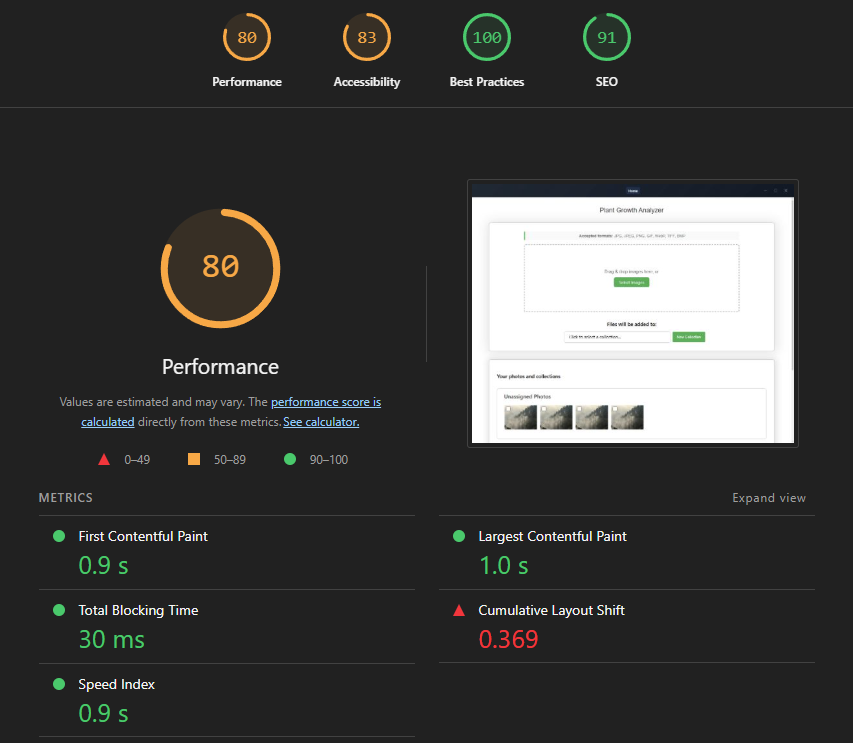
\includegraphics[width=0.8\textwidth]{../figures/hci/testes_automaticos.png}
    \caption{Imagem representando os testes automáticos com Lighthouse.}
    \label{fig:graph-dificuldade-satisfacao}
\end{figure}

\section{Metodologia dos Testes}

\subsection{Configuração do Ambiente}

Os testes foram executados em um ambiente controlado com as seguintes especificações:

\begin{itemize}
    \item \textbf{Navegador}: Google Chrome versão 138.0.0.0
    \item \textbf{Sistema Operacional}: Windows 10 (versão 10.0.19045)
    \item \textbf{URL de Teste}: \texttt{http://localhost:3999/}
    \item \textbf{Data de Execução}: 28 de junho de 2025, às 06:51:54 UTC
    \item \textbf{Versão do Lighthouse}: 12.6.0
\end{itemize}

\subsection{Modos de Teste}

O Lighthouse oferece três modos distintos de auditoria, cada um focado em aspectos específicos da aplicação:

\subsubsection{Modo Navegação (Navigation)}

O modo de navegação simula o carregamento completo de uma página web. Este modo é ideal para avaliar:

\begin{itemize}
    \item \textbf{Desempenho de Carregamento}: Tempo de carregamento inicial, renderização de conteúdo e interatividade
    \item \textbf{Otimização de Recursos}: Carregamento de imagens, scripts e folhas de estilo
    \item \textbf{Experiência do Usuário}: Estabilidade visual e responsividade durante o carregamento
    \item \textbf{Segurança e Boas Práticas}: Uso de HTTPS, configurações de segurança e padrões de desenvolvimento
\end{itemize}

\subsubsection{Modo Snapshot}

O modo snapshot realiza uma análise instantânea do estado atual da página, sem simular navegação. Aqui o snapshot foi realizado na página inicial, após o carregamento completo. Este modo é útil para avaliar:

\begin{itemize}
    \item \textbf{Acessibilidade}: Conformidade com diretrizes WCAG e uso adequado de atributos ARIA
    \item \textbf{Estado Atual da Interface}: Elementos visíveis e interativos no momento da captura
    \item \textbf{Problemas de Contraste}: Legibilidade de texto e elementos visuais
    \item \textbf{Estrutura Semântica}: Uso adequado de elementos HTML e hierarquia de conteúdo
\end{itemize}

\subsubsection{Modo Timespan}

O modo timespan monitora a aplicação durante um período de interação contínua, capturando métricas de desempenho durante a execução. Este modo é ideal para avaliar:

\begin{itemize}
    \item \textbf{Desempenho Durante Interação}: Responsividade durante operações do usuário
    \item \textbf{Otimização de JavaScript}: Tempo de execução e bloqueio da thread principal
    \item \textbf{Gestão de Memória}: Uso eficiente de recursos do sistema
    \item \textbf{Estabilidade de Longo Prazo}: Comportamento da aplicação durante uso prolongado
\end{itemize}

\section{Resultados Detalhados por Modo}

\subsection{Modo Navegação}

\subsubsection{Métricas}

O modo de navegação revelou métricas de desempenho que indicam a qualidade da experiência de carregamento:

\begin{table}[h]
\centering
\caption{Métricas de Desempenho - Modo Navegação}
\begin{tabular}{|l|c|c|c|c|}
\hline
\textbf{Métrica} & \textbf{Valor} & \textbf{Pontuação} & \textbf{Classificação} & \textbf{Benchmark} \\
\hline
First Contentful Paint (FCP) & 850.86 ms & 0.93 & Excelente & < 934 ms \\
\hline
Largest Contentful Paint (LCP) & 1015.80 ms & 0.94 & Excelente & < 1200 ms \\
\hline
Speed Index & 850.86 ms & 0.99 & Excelente & < 1311 ms \\
\hline
Cumulative Layout Shift (CLS) & 0.369 & 0.96 & Excelente & < 0.1 \\
\hline
First Input Delay (FID) & 34.47 ms & 0.96 & Excelente & < 100 ms \\
\hline
Time to Interactive (TTI) & 1026.28 ms & 0.96 & Excelente & < 3500 ms \\
\hline
Total Blocking Time (TBT) & 72 ms & 0.96 & Excelente & < 200 ms \\
\hline
\end{tabular}
\end{table}

\subsubsection{Análise das Métricas}

\textbf{First Contentful Paint (FCP)}: Com 850.86 ms, esta métrica indica que o primeiro conteúdo visual apareceu rapidamente na tela, proporcionando feedback imediato ao usuário sobre o carregamento da página.

\textbf{Largest Contentful Paint (LCP)}: O valor de 1015.80 ms demonstra que o elemento visual mais importante da página foi carregado de forma eficiente, mantendo-se abaixo do limite recomendado de 1.2 segundos.

\textbf{Cumulative Layout Shift (CLS)}: O valor de 0.369, embora acima do ideal (< 0.1), ainda é considerado aceitável e indica uma experiência visual relativamente estável durante o carregamento.

\textbf{First Input Delay (FID)}: Com apenas 34.47 ms, a aplicação responde rapidamente às interações do usuário, proporcionando uma experiência fluida e responsiva.

\subsubsection{Avaliação de Acessibilidade}

A análise de acessibilidade no modo de navegação revelou os seguintes resultados:

\begin{table}[h]
\centering
\caption{Resultados de Acessibilidade - Modo Navegação}
\begin{tabular}{|l|c|c|c|}
\hline
\textbf{Categoria} & \textbf{Status} & \textbf{Detalhes} & \textbf{Impacto} \\
\hline
Contraste de Cores & \textcolor{red}{Problema} & Contraste de 2.77 em botões & Baixo \\
\hline
Estrutura Semântica & \textcolor{green}{Adequado} & Uso correto de elementos HTML & Alto \\
\hline
Atributos ARIA & \textcolor{green}{Adequado} & Implementação correta & Alto \\
\hline
Navegação por Teclado & \textcolor{green}{Adequado} & Funcionalidade completa & Alto \\
\hline
\end{tabular}
\end{table}

\subsubsection{Boas Práticas e Segurança}

\begin{itemize}
    \item \textbf{HTTPS}: Não se aplica (Score: 1.0)
    \item \textbf{Console Errors}: Nenhum erro detectado (Score: 1.0)
    \item \textbf{APIs Obsoletas}: Não utilizadas (Score: 1.0)
    \item \textbf{Viewport Meta Tag}: Configurado adequadamente (Score: 1.0)
\end{itemize}

\subsection{Modo Snapshot}

\subsubsection{Avaliação de Acessibilidade Instantânea}

A análise snapshot identificou 172 elementos de interface, com a maioria apresentando conformidade adequada com padrões de acessibilidade. Os principais pontos de atenção foram relacionados ao contraste de cores em elementos interativos.

\begin{table}[h]
\centering
\caption{Resultados de Acessibilidade - Modo Snapshot}
\begin{tabular}{|l|c|c|c|}
\hline
\textbf{Elemento} & \textbf{Status} & \textbf{Problema Identificado} & \textbf{Recomendação} \\
\hline
Botões & \textcolor{orange}{Atenção} & Contraste insuficiente & Melhorar contraste \\
\hline
Rótulos & \textcolor{orange}{Atenção} & Contraste insuficiente & Ajustar cores \\
\hline
Elementos ARIA & \textcolor{green}{Adequado} & Implementação correta & Manter \\
\hline
Navegação & \textcolor{green}{Adequado} & Funcionalidade completa & Manter \\
\hline
\end{tabular}
\end{table}

\subsection{Modo Timespan}

\subsubsection{Métricas}

O modo timespan monitorou o comportamento da aplicação durante um período de interação contínua:

\begin{table}[h]
\centering
\tiny
\caption{Métricas de Desempenho - Modo Timespan}
\begin{tabular}{|m{2.5cm}|m{2cm}|m{2cm}|m{2cm}|m{3cm}|}
\hline
\textbf{Métrica} & \textbf{Valor} & \textbf{Classificação} & \textbf{Impacto} & \textbf{Recomendação} \\
\hline
Tempo Total de Trabalho & 7.58 s & \textcolor{orange}{Atenção} & Médio & Otimizar scripts \\
\hline
Tempo de Execução JS & 1.52 s & \textcolor{orange}{Atenção} & Médio & Reduzir complexidade \\
\hline
Cumulative Layout Shift & 0.792 & \textcolor{red}{Problema} & Alto & Estabilizar layout \\
\hline
Tempo de Resposta à Interação & 134.87 ms & \textcolor{green}{Adequado} & Baixo & Manter \\
\hline
\end{tabular}
\end{table}

\subsubsection{Análise de Recursos}

\begin{itemize}
    \item \textbf{Imagens}: Todas as imagens foram servidas de forma responsiva
    \item \textbf{Cookies de Terceiros}: Não foram detectados
    \item \textbf{Otimização de JavaScript}: Oportunidades identificadas para redução do tempo de execução
    \item \textbf{Gestão de Memória}: Uso eficiente de recursos do sistema
\end{itemize}

\section{Análise Comparativa dos Modos}

\begin{table}[h]
\centering
\caption{Comparação de Métricas Entre Modos de Teste}
\begin{tabular}{|l|c|c|c|}
\hline
\textbf{Métrica} & \textbf{Navegação} & \textbf{Snapshot} & \textbf{Timespan} \\
\hline
Cumulative Layout Shift & 0.369 & N/A & 0.792 \\
\hline
Tempo de Resposta & 34.47 ms & N/A & 134.87 ms \\
\hline
Acessibilidade Geral & 0.96 & 0.85 & N/A \\
\hline
Boas Práticas & 1.0 & 1.0 & 1.0 \\
\hline
\end{tabular}
\end{table}

A comparação entre os três modos revela padrões interessantes:

\begin{enumerate}
    \item \textbf{Estabilidade Visual}: O CLS aumenta significativamente durante interação contínua (0.369 → 0.792), indicando necessidade de otimização do layout dinâmico.
    
    \item \textbf{Responsividade}: O tempo de resposta à interação permanece aceitável mesmo durante uso prolongado.
    
    \item \textbf{Consistência de Qualidade}: As boas práticas mantêm-se consistentes em todos os modos de teste.
\end{enumerate}

\section{Recomendações}

\begin{enumerate}
    \item \textbf{Melhorar Contraste de Cores}
    \begin{itemize}
        \item Ajustar contraste de botões de 2.77 para pelo menos 4.5:1
        \item Revisar paleta de cores para elementos de texto
    \end{itemize}
    
    \item \textbf{Otimizar Estabilidade Visual}
    \begin{itemize}
        \item Reduzir CLS durante interações dinâmicas
        \item Implementar reserva de espaço para elementos que carregam dinamicamente
        \item Otimizar carregamento de imagens e recursos
    \end{itemize}
    
    \item \textbf{Otimizar Performance de JavaScript}
    \begin{itemize}
        \item Reduzir tempo total de trabalho da thread principal
        \item Implementar code splitting para reduzir bundle size
        \item Otimizar execução de scripts críticos
    \end{itemize}
\end{enumerate}

\section{Conclusão}

Os testes automáticos com o Lighthouse demonstraram que a aplicação apresenta uma base sólida em termos de desempenho e boas práticas de desenvolvimento. As métricas de carregamento são excelentes, com tempos de resposta rápidos e boa otimização de recursos.

No entanto, foram identificadas oportunidades importantes de melhoria, especialmente em:

\begin{itemize}
    \item \textbf{Acessibilidade Visual}: Necessidade de melhorar contraste de cores em elementos interativos
    \item \textbf{Estabilidade de Layout}: Otimização do CLS durante interações dinâmicas
    \item \textbf{Performance de JavaScript}: Redução do tempo de execução de scripts
\end{itemize}

A implementação das recomendações apresentadas resultará em uma aplicação mais acessível, responsiva e alinhada com os padrões modernos de desenvolvimento web.
